\documentclass[basic,plain]{inVerba-notes}
\usepackage{inVerba-math}

\newcommand{\userName}{Cullyn Newman}
\newcommand{\class}{BI:\@ 337}
\newcommand{\theTitle}{Lab 2: Cellular Transport}
\newcommand{\institution}{Portland State University}

\begin{document}

\begin{center}
  {\Large\textbf{\rrr{Description of Techniques} and \bbb{Explanation of Concepts}}}
\end{center}

\hrule
\medskip

{\large\textbf{Optogenetic Stimulation Induced Attack}}
\begin{itemize}
  \item ``We next tested whether \bbb{functional manipulations of VMHvl would affect mating or fighting\(^1\)}. Although VMHvl overlaps the rat HAA, extensive attempts to elicit attack by conventional electrical stimulation of this region in mice were unsuccessful. As an alternative, therefore, we \rrr{expressed channelrhodopsin-2 (ChR2) in VMHvl neurons unilaterally\(^1\)}, using stereotactic \rrr{co-injection of adeno-associated viral vectors (AAV2)\(^2\)} expressing Cre recombinase and a Cre-dependent form of ChR2 fused with enhanced yellow fluorescent protein (ChR2–EYFP) and \bbb{selectively illuminated cells\(^2\)} in this region \rrr{using an implanted fibreoptic cable (Fig. 4a)\(^3\)}.
  
  \begin{center}
    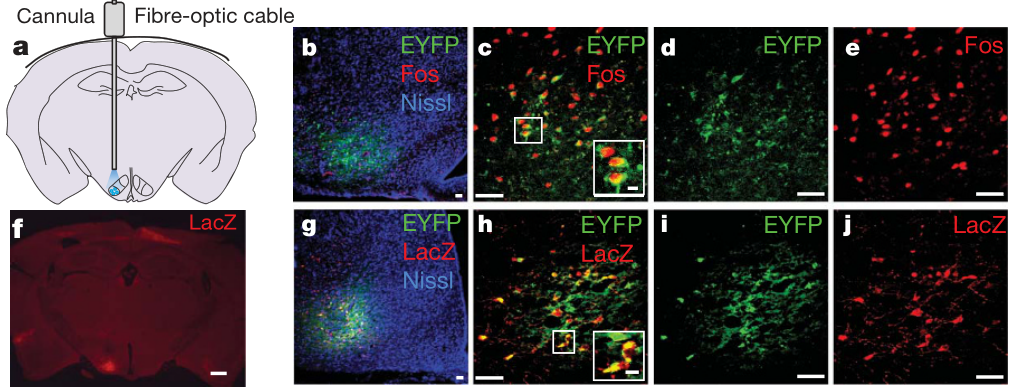
\includegraphics[width=0.9\textwidth]{images/week-2-a.png}
  \end{center}
    \begin{itemize}
      \item \bbb{Hypothesis in question\(^1\)}: this section deals with figure 4 in the paper, where the authors are testing whether functional manipulations of VMHvl are affect behavior, but had an issue of selectively activating the area. 
      \item \rrr{ChR2\(^2\)}: use of channelrhodopsin (light gated ion channels), specifically channelrhodopsin-2, allowed the researcher to \bbb{select particular neurons\(^2\)} to analyze cell responses in VMHv1 directly.
      \item \rrr{Co-injection of AAV2\(^3\)}: AAV2 infects neurons preferentially, allowing only neurons whose cell bodies are local to the injection site express the CHR2. Co-injection ensures that cells observed are exactly the neurons in question, which blue region under \tbm{a} in the above image.
    \end{itemize}
    \item \bbb{Selectively illuminated cells\(^2\)} \rrr{using an implanted fibreoptic cable\(^3\)}: ``results showed that \textit{c-fos} could be strongly induced in VMHvl on the infected, but not the contralateral control side after repeated blue light stimulation in awake animals.''
    \begin{itemize}
      \item The actual analysis of how the authors determined this result is something I'm struggling to understand. I get the idea of injecting and selectively controlling regions that respond to the optogenetic light, allowing for functional testing of behavior, but I don't \tbm{b}--\tbm{e} and \tbm{g}--\tbm{h}. 
      \item \tbm{f}: does use LacZ to identify infected cell bodies, which I assume is to verify effectiveness of AAV2.
    \end{itemize}
\end{itemize}

\end{document}